%! Author = danielmendes
%! Date = 15.02.25

\chapter{Partitionen}\label{ch:partitions}

In diesem Kapitel wird die Funktionsweise von Partitionen und das Verhalten des Abfrageoptimierers untersucht.
Partitionierte Datenbanken existieren bereits seit den 1980er Jahren, haben jedoch in jüngerer Zeit durch NoSQL-Datenbanken und Hadoop-basierte Data Warehouses eine erneute Aufmerksamkeit erfahren (vgl.\ \cite[S. 200]{kleppmann2017designing}).
Auch in relationalen Datenbanken besteht die Möglichkeit, Daten auf verschiedene Partitionen zu verteilen.
In MySQL stehen dabei verschiedene Partitionierungstypen zur Verfügung, darunter RANGE-, LIST-, HASH- und KEY-Partitionierung.
Für jeden dieser Typen werden Anwendungsbeispiele präsentiert und mögliche Verwendungszwecke erläutert.
Abschließend werden Benchmark-Tests durchgeführt, um die jeweiligen Vor- und Nachteile zu bewerten.


\section{Grundlagen}\label{sec:partition-grundlagen}

Zunächst muss geklärt werden, was mit Partitionen gemeint ist.

\begin{quote}
	\enquote{Partitioning is a general term used to describe the act of breaking up data and distributing it across different hosts.} (\cite[S. 148]{da2015redis})
\end{quote}

In NoSQL-Datenbanken werden diese Partitionen häufig auf verschiedene Server verteilt, können jedoch auch innerhalb eines einzelnen Servers gespeichert werden.
Im Gegensatz dazu bezieht sich die Partitionierung in MySQL ausschließlich auf die Verteilung von Tabellendaten innerhalb einer einzigen Datenbankinstanz.
Dabei werden die Daten auf verschiedene physische oder logische Partitionen innerhalb desselben Servers verteilt.
Zur Verteilung auf mehrere Server kann in relationalen Datenbanken Replikation eingesetzt werden, die im nächsten Kapitel~\ref{ch:partitions} ausführlicher erläutert wird.
Das System verwaltet sie intern so, dass der Benutzer nicht bemerkt, wie genau die Daten organisiert sind (\cite[S. 265--273]{schwartz2012high}).
Damit eine Tabelle die Partitionierung nutzt, muss bei ihrer Erstellung die \texttt{PARTITION BY}-Klausel angegeben werden, die festlegt, in welcher Partition jede Datenzeile gespeichert wird.
Dies führt zu einer erhöhten Komplexität des \texttt{CREATE TABLE}-Befehls.
In der Partitionsklausel selbst können nicht nur Ausdrücke und Berechnungen zur Bestimmung der Partitionierung eingesetzt werden, sondern auch Funktionen.
Wenn Funktionen verwendet werden, müssen sie eine nicht-konstante und deterministische Ganzzahl zurückgeben, wie z.B. \texttt{YEAR()}.

Um Partitionen ordnungsgemäß definieren zu können, sind bestimmte Einschränkungen zu beachten.
Zum einen müssen alle Spalten, nach denen die Partitionierung erfolgt, im Primärschlüssel oder Unique-Index enthalten sein.
Andernfalls ist es nicht möglich, die Partitionen korrekt zu erstellen oder zu verwalten.
Als logische Schlussfolgerung ergibt sich ein zusätzlicher Aufwand für die Pflege der neuen Indizes.
Zudem können Fremdschlüssel-Bedingungen (engl.\ foreign key constraints) nicht verwendet werden.
Ein weiteres Limit betrifft die maximale Anzahl an Partitionen pro Tabelle.
Bei älteren MySQL-Versionen liegt dieses Limit bei 1024 und seit der MySQL-Version 8.0 bei 8192 Partitionen (\cite{mysql_nof_partitions}).
Wie später noch festgestellt wird, sollte aus verschiedenen Gründen die Anzahl der Partitionen so gering wie möglich gehalten werden.
Aus diesem Grund ist diese Grenze nicht sehr relevant, sollte sie dennoch beachtet werden.

Nachdem die grundlegenden Bedingungen nun geklärt sind, wird im Folgenden die Funktionsweise erläutert.
Wie bereits erwähnt, bestehen partitionierte Tabellen aus mehreren zugrunde liegenden Tabellen, die durch sogenannte Handler-Objekte verwaltet werden.
Das Handler-Objekt fungiert als Schnittstelle, die es dem Datenbankmanagementsystem ermöglicht, mit den Partitionen zu interagieren.
Dabei leitet es Anfragen an die Storage Engine weiter, die die Daten verwaltet.
Aus Sicht der Storage Engine sind Partitionen normale Tabellen, unabhängig davon, ob sie eigenständig oder Teil einer partitionierten Tabelle sind.
Abhängig vom jeweiligen Datenbankmanagementsystem können einzelne Partitionen entweder direkt oder, wie beispielsweise in MySQL, nicht direkt angesprochen werden.
In Oracle ist dies wie folgt möglich:

\vspace{-5pt}
\begin{lstlisting}[language=SQL,label={lst:direct_partition}]
SELECT * FROM your_table PARTITION (your_partition_name);
\end{lstlisting}
\vspace{-7pt}

Die Verwendung von Indizes bei der Partitionierung wird von den verschiedenen DBMS unterschiedlich gehandhabt.
In MySQL werden Indizes für jede Partition separat definiert, anstatt sie über die gesamte Tabelle hinweg zu erstellen.
Dabei werden die Indizes identisch auf jede Partition angewendet.
In Oracle hingegen gibt es neben den lokalen Indizes auch globale, die über die gesamte Tabelle hinweg erstellt werden, unabhängig von den Partitionen.
Diese Methode ermöglicht eine effizientere Suche, erfordert jedoch eine komplexere Verwaltung.

Als Nächstes ist es wichtig zu verstehen, wie der Abfrageoptimierer (engl.\ Query Optimizer) arbeitet.
Beim Ausführen von Abfragen versucht er, überflüssige Partitionen auszuschließen und sich gezielt auf diejenigen zu konzentrieren, die die relevanten Daten enthalten.
Damit das sogenannte Pruning funktioniert, muss die \texttt{WHERE}-Klausel mit dem Partitionsausdruck übereinstimmen.
Der Query Optimizer entscheidet bei SELECT-Abfragen, welche Partitionen ignoriert werden können und leitet die Anfrage gezielt weiter.
Bei DELETE-Abfragen wird die betroffene Zeile lokalisiert und die Anfrage an die passende Partition übermittelt.
Für INSERT-Abfragen wird zunächst die Zielpartition für die neue Zeile ermittelt.
Erfolgt ein UPDATE innerhalb einer Partition, wird die Anfrage ebenfalls an die jeweilige Partition übermittelt.
Wenn aber Teile der Partitionslogik verändert werden, dann stellt UPDATE eine Kombination von INSERT und DELETE dar, da eine Einfügungsanfrage an die Zielpartition und eine Löschanfrage an die Quellpartition weitergeleitet wird.
Die meisten dieser Operationen unterstützen Pruning, während, einige, wie z.B.\ INSERT-Abfragen von Natur aus ausschließend (engl.\ self-pruned) sind.
Durch die Funktionsweise des Pruning lassen sich schon einige Vorteile der Partitionierung erkennen, die im Folgenden näher betrachtet werden.

Wie bei der Indexierung und der Datenclusterung einer Tabelle, trägt Partitionierung dazu bei, große Teile der Tabelle vom Zugriff auszuschließen und zusammengehörige Zeilen nahe beieinander zu speichern.
Daher bietet es sich an, anstelle von indexierten Tabellen partitionierte Strukturen zu verwenden, um einen schnellen Zugriff auf die gewünschten Zeilen zu ermöglichen.
Durch die korrekte Verteilung der Partitionen befindet man sich, wie bei Indizes, nahe der gewünschten Daten und kann von dort aus entweder das relevante Datengebiet sequentiell scannen oder es in den Speicher laden und indexieren.
Im Gegensatz zu Indizes hat die Partitionierung aber zwei entscheidende Vorteile.
Zum einen ist keine separate Datenstruktur erforderlich, auf die verwiesen werden muss und die ständig aktualisiert wird, wodurch nur geringer Mehraufwand verursacht wird.
Stattdessen gibt es eine mathematische Formel, die bestimmt, welche Partitionen welche Kategorien von Zeilen enthalten können.
Zum anderen lassen sich auch physisch verteilen, sodass der Server mehrere Festplatten effizienter nutzen kann.
Besonders vorteilhaft ist dies, wenn die Tabellen sehr groß sind und nicht mehr vollständig in den Speicher passen.

\begin{quote}
	\enquote{The goal of partitioning is to spread the data and query load evenly across multiple machines, avoiding hot spots (nodes with disproportionately high load).} (\cite[S. 217]{kleppmann2017designing})
\end{quote}

Außerdem steigt die Effizienz der Partitionierung, je mehr Partitionen durch die \texttt{WHERE}-Klausel in der Abfrage ausgeschlossen werden.
Die Effizienz basiert aber auf zwei wesentlichen Annahmen.
Erstens muss die Suche durch das Pruning von Partitionen bei der Abfrage eingegrenzt werden können.
Zweitens darf die Partitionierung selbst keine hohen Kosten verursachen.
Diese Annahmen sind jedoch nicht immer gültig, weshalb drei Anwendungsfälle mit möglichen Fehlern im Umgang mit Partitionen vorgestellt werden.

Zunächst sollte berücksichtigt werden, dass das Ergebnis einer Partitionierungsfunktion, wie z.B.\ \texttt{YEAR()}, den Wert \texttt{NULL} annehmen kann.
Selbst wenn eine zeitbasierte Spalte als \texttt{NOT NULL} deklariert wird, können ungültige Datumswerte auftreten, die in MySQL in der ersten definierten Partition gespeichert werden.
Eine Abfrage, die Jahre außer 2020 herausfiltert, muss daher zwei Partitionen durchsuchen, was insbesondere größeren Partitionen die Performance beeinträchtigt.
Aus diesem Grund empfiehlt es sich, entweder eine dedizierte Partition für solche Sonderfälle einzuführen oder Erweiterung wie \texttt{RANGE COLUMNS} verwenden, die auf Funktionen in der Partitionsdefinition verzichten.
Des Weiteren muss man bei der Definition von Indizes vorsichtig sein, wenn diese nicht mit der Partitionsklausel übereinstimmen, da sie unerwartet zu umfassenderen Suche der Partitionen führen können.
Daher sollte man es vermeiden, Indizes auf nicht partitionierten Spalten zu erstellen.
Dies gilt nur dann nicht, wenn sichergestellt ist, dass die Abfragen Ausdrücke enthalten, die das Pruning der Partitionen unterstützen.
Zuletzt sollte die Anzahl der definierten Partitionen begrenzt werden, da der Server die Partitionsdefinitionen linear durchsuchen muss, was mit steigender Partitionenzahl zunehmend ineffizient wird.
Zusätzlich entsteht ein nicht vermeidbarer Mehraufwand durch das Öffnen und Sperren von Partitionen vor dem Pruning, was die Abfrageleistung weiter beeinträchtigen kann.
Wie genau die Partitionen für die verschiedenen Typen definiert werden können, wird im Folgenden erläutert.

\section{Arten der Partitionierung}\label{sec:arten-der-partitionierung}

In diesem Unterkapitel werden die verschiedenen Partitionierungsarten, die von MySQL unterstützt werden, jeweils mit einem Beispiel näher erläutert.
Die Analyse der Ergebnisse erfolgt in Abschnitt~\ref{sec:partition-analyse}.

Als Grundlage dienen die Kundentabelle (\ref{lst:tools-create-table-kunde}) und die Bestelltabelle (\ref{lst:tools-create-table-bestellung}), die bereits in früheren Kapiteln verwendet wurden.
Die Tabelle, die auf unterschiedliche Partitionen verteilt werden soll, ist die Kundentabelle.
Allerdings müssen beide Tabellen noch angepasst werden, da es auch Einschränkungen für partitionierte Tabellen gibt.
Zum einen muss bei der Bestelltabelle bei allen Typen die Fremdschlüssel-Bedingung entfernt werden und zum anderen muss der Primärschlüssel der Kundentabelle angepasst werden.
Wie genau das passieren muss, wird an den Beispielen ersichtlich.
Die Insert-Befehle sind bei allen Typen der Partitionierung gleich, bei den Select-Queries gibt es jedoch Unterschiede.

Der erste Typ, der betrachtet wird, ist die RANGE-Partitionierung.
Bei dieser erfolgt die Zuordnung von Zeilen zu Partitionen basierend auf Spaltenwerten, die in einen definierten Wertebereich fallen.
Für das Beispiel sollen unterschiedliche Partitionen je nach Alter des Kunden gebildet werden.
Alle fünf Jahre wird eine neue Partition gebildet.

Damit es zu keinen Fehlern kommt, muss hier der Geburtstag auch Teil des Primärschlüssels der Kundentabelle sein.
Außerdem muss die Spalte \texttt{GEBURTSTAG} bei der Bestelltabelle hinzugefügt werden, damit das Joinen der Tabellen über den Primärschlüssel effizienter ist.
Seit MySQL 5.5 kann für Datumsspalten auch die Erweiterung \texttt{RANGE COLUMNS} verwendet werden, wodurch bei der Partitionsklausel die Funktion \texttt{YEAR()} nicht erforderlich ist.
Um die Performance der beiden Ansätze zu vergleichen, werden beide Varianten bei der Tabellenerstellung verwendet.
Die Tabelle mit der Funktion \texttt{YEAR{}} wird wie folgt erstellt:

\lstinputlisting[
	language=sql,
	caption=Kundetabelle mit Range-Partitionierung,
	label={lst:create_kunden_partition_range},
	style=custom_daniel,
]{Scripts/Partition/01_Create_Kunden_Partition_Range.sql}
\vspace{-5pt}

Bei der Range-Partitionierung werden mehrere Select-Befehle getestet, da das Pruning je nach Art der Datumsabfrage besser oder schlechter funktioniert (siehe Abschnitt~\ref{sec:partition-grundlagen}).
Dazu wird zunächst die Kundentabelle mit der Bestelltabelle über die Attribute \texttt{KUNDEN\_ID} und \texttt{GEBURTSTAG} gejoint.
Die Testkunden werden so generiert, dass sie immer zufällig zwischen den Jahren 1950 und 2020 geboren sind.
Die verschiedenen Select-Befehle unterscheiden sich in den folgenden \texttt{WHERE}-Bedingungen:

\vspace{-5pt}
\begin{lstlisting}[language=SQL,caption=Unterschiedliche WHERE-Bedingungen,label={lst:different_where_conditions}]
WHERE YEAR(k.GEBURTSTAG) = 1985;		             -- failing_pruning.sql
WHERE k.GEBURTSTAG BETWEEN '1985-01-01' AND '1985-12-31'; 	-- with_pruning.sql
WHERE k.GEBURTSTAG = '1985-01-01';		            -- with_primary_key.sql
\end{lstlisting}
\vspace{-5pt}

Um zu überprüfen, ob der Optimierer die Partitionen pruned, wird der SQL-Befehl \texttt{EXPLAIN} vor dem \texttt{SELECT}-Befehl in~\ref{lst:different_where_conditions} verwendet.
Als Rückgabe des Befehls erhält man eine Übersicht, wie MySQL die Abfrage ausführt und welche Partitionen dabei verwendet wurden.
Zunächst wird eine Select-Query analysiert, bei der keine \texttt{WHERE}-Klausel angegeben ist.
Im Ergebnis von \texttt{EXPLAIN} sehen wir, dass der Abfragemechanismus alle Partitionen durchsuchen muss.
Bei der \texttt{WHERE}-Klausel der Abfrage in Zeile 1 wird eigentlich erwartet, dass nur eine Partition abgefragt wird, jedoch wird das gleiche Resultat wie bei der vorherigen Abfrage zurückgegeben.
Die Query aus der zweiten Zeile verweist direkt auf die Partitionsspalte und nicht auf einen Ausdruck.
Und tatsächlich wird hier nur die Partition untersucht, die alle Kunden mit Geburtsdaten zwischen den Jahren 1985 und 1990 enthält.
Diese Partition wird auch ausschließlich in der Abfrage der letzten Zeile benutzt.
Daraus lässt sich schließen, dass MySQL nur dann Partitionen effizient prunen kann, wenn die Abfrage direkt auf die Partitionsspalte zugreift und keine Ausdrücke verwendet.
Dieses Verhalten ähnelt dem von indexierten Spalten, die ebenfalls im Abfrageausdruck isoliert sein müssen, damit der Index zum Einsatz kommt.

Als Nächstes wird die LIST-Partitionierung betrachtet, bei der die Partitionen anhand von Spaltenwerten ausgewählt werden, die einem der vordefinierten diskreten Werte entsprechen.
Zur Veranschaulichung soll pro Land eine eigene Partition erstellt werden.
Dafür muss die Spalte \texttt{LAND} Teil des Primärschlüssels sein.
Beim Befüllen der Tabellen wird für jeden Kunden ein zufälliges Land aus der Liste der 20 einwohnerreichsten Länder der Welt ausgewählt.
Daher müssen bei der Erstellung der Tabelle auch 20 Partitionen sowie eine zusätzliche für sonstige Werte erstellt werden (\ref{lst:create_kunden_partition_list}).

\vspace{-5pt}
\lstinputlisting[
	language=sql,
	caption=Kundetabelle mit List-Partitionierung,
	label={lst:create_kunden_partition_list},
	style=custom_daniel,
]{Scripts/Partition/02_Create_Kunden_Partition_List.sql}
\vspace{-5pt}

Im Rahmen der List-Partitionierung wird ebenfalls die Performance unterschiedlicher Select-Befehle überprüft.
Zunächst wird, wie zuvor, die Kundentabelle mit der Bestelltabelle gejoint.
Anschließend wird in der \texttt{WHERE}-Bedingung aber so gefiltert, dass nur Kunden aus Deutschland ausgewählt werden.
Zusätzlich soll die Performance untersucht werden, wenn aus der Liste der Länder zufällig fünf ausgewählt werden und alle Kunden nur aus einem dieser fünf Länder stammen.
Dazu werden drei verschiedene Ansätze getestet.
Zum einen über den \texttt{OR}-Operator, zum anderen mithilfe des \texttt{IN}-Operators und zuletzt werden die 5 Länder, wie im ersten Beispiel, einzeln abgefragt und die Ergebnisse der 5 Abfragen mithilfe des \texttt{UNION}-Operators verbunden.
Mithilfe von \texttt{EXPLAIN} wird sichtbar, dass bei allen Varianten nur die Partitionen der 5 Länder genutzt werden.
Damit kann der Optimierer Bereiche in Listen diskreter Werte umwandeln, Elemente prunen und während der Abfrageverarbeitung Partitionen gezielt entfernen.
Im Zusammenhang mit Joins ist der Effekt besonders stark, da MySQL bei einem partitionierten Schlüssel in der Join-Bedingung nur in den relevanten Partitionen nach übereinstimmenden Zeilen sucht.
Welche der Varianten jedoch am effizientesten ist, wird erst bei der Analyse ersichtlich sein.

Zum Schluss wird die HASH-Partitionierung betrachtet, bei der die Partition anhand eines Hash-Werts zugewiesen wird, der aus den Spaltenwerten der Zeilen berechnet wird.
Dadurch kann eine gleichmäßige Verteilung der Daten auf die Partitionen werden.

\begin{quote}
	\enquote{Because of this risk of skew and hot spots, many distributed datastores use a hash function to determine the partition for a given key.} (\cite[S. 203]{kleppmann2017designing})
\end{quote}

Zur Umsetzung der Tabelle müssen ausschließlich die Zeilen aus dem Codeblock~\ref{lst:create_kunden_partition_hash} am Ende des Create-Kunden-Befehls hinzugefügt werden.
In diesem Fall wird auch nur eine einzige Select-Query getestet, die wieder beide Tabellen joined und in der \texttt{WHERE}-Bedingung überprüft, ob die \texttt{KUNDEN\_ID} zwischen den Werten 1000 und 2000 liegt.
Um mehr Werte miteinander zu vergleichen, werden verschiedene Varianten der Hash-Partitionierung getestet, indem die Anzahl der Partitionen variiert wird.
Die Anzahl der Partitionen beträgt in den Benchmarks 5, 50 und 500.
Einschließlich des Referenzfalls ergeben sich somit vier unterschiedliche Testfälle, die miteinander verglichen werden.

\vspace{-7pt}
\begin{lstlisting}[language=SQL,caption=Hash-Partitonierung,label={lst:create_kunden_partition_hash}]
PARTITION BY HASH(KUNDEN_ID)
PARTITIONS 5;
\end{lstlisting}
\vspace{-5pt}

Die KEY-Partitionierung ähnelt der Hash-Partitionierung, verwendet jedoch die interne Hash-Funktion von MySQL und benötigt nur die Angabe einer oder mehrerer Spalten.
Um die Performance zu überprüfen, wird genau das Gleiche wie bei der Hash-Partitionierung gemacht.
Dafür muss im Codeblock~\ref{lst:create_kunden_partition_hash} das Signalwort \texttt{HASH} mit \texttt{KEY} ersetzt werden und das Ergebnis wird mit dem von \texttt{HASH} verglichen.
Die Erkenntnisse aus diesem Benchmark werden im nächsten Kapitel zusammengefasst.

\section{Analyse}\label{sec:partition-analyse}

Im vorherigen Abschnitt wurden die verschiedenen Arten von Partitionen erläutert.
Nun sollen für jedes dieser Beispiele Benchmarks durchgeführt und die Ergebnisse untersucht werden.
Um den Einfluss der Partitionierung auf die Abfragen zu verdeutlichen, werden jeweils partitionierte mit nicht partitionierten Tabellen verglichen.
Beide Varianten stellen die gleichen Insert-Befehle, während sich die Select-Queries je nach Partitionierungstyp leicht unterscheiden können.
Abhängig vom Typ werden zusätzlich leicht unterschiedliche Abfragen gestellt.
Die Ergebnisse des Referenzbenchmarks sollten weitgehend mit denen der partitionierten Varianten übereinstimmen.
Es können jedoch kleinere Unterschiede auftreten, da jeweils zufällig generierte Daten eingefügt werden.
Bei signifikanten Abweichungen sind die Performancemessungen jedoch schwerer miteinander vergleichbar.

Im ersten Benchmark mit der Range-Partitionierung fällt auf, dass die Benutzung von \texttt{RANGE} oder \texttt{RANGE COLUMNS} keinerlei Einfluss auf die Performance hat.
Daher stellt sich bei der Verwendung nicht die Frage nach der Performance, sondern nach der Präferenz des Nutzers.
Bei der Analyse der Abbildung~\ref{fig:range-partition} wird deutlich, dass die \texttt{with\_pruning}-Query mit erheblichem Abstand schneller ist als die anderen.
Damit funktioniert das Pruning besonders gut, wenn die Geburtstage zwischen dem ersten und letzten Tage des Jahres abfragen.
Als Nächstes kommen die Skripte ohne Partitionierung, die aber etwa 50\% ineffizienter sind, als das Skript zuvor.
Da beide auf einem sehr ähnlichen Niveau liegen, kann davon ausgegangen werden, dass die Verarbeitung durch \texttt{YEAR()} hier keine Rolle spielt.
Etwas langsamer bei der Range-Partitionierung ist \texttt{with\_primary\_key}, bei der nur die Kunden abgerufen werden, die am 1.\ Januar 1985 geboren wurden.
Wenn die Ergebnisse von \texttt{EXPLAIN} betrachtet werden, zeigt sich, dass bei der Abfrage nur eine Partition verwendet wurde.
Als Letztes kommen die beiden Select-Queries, die alle Partitionen durchsuchen.
Bei der einen Abfrage wurde keine \texttt{WHERE}-Bedingung angegeben und bei der anderen wurde die Funktion \texttt{YEAR()} verwendet.
Es lässt sich also feststellen, dass Pruning mithilfe von \texttt{YEAR()} offensichtlich nicht funktioniert.
Dies hat auch der Ausführungsplan für die Query bestätigt (siehe Kapitel~\ref{sec:arten-der-partitionierung}).
Bei den Insert-Befehlen ist der Fall ohne Partitionierung nur geringfügig schneller als mit Partitionierung.

\vspace{-7pt}
\begin{figure}[H]
	\centering
	\begin{subfigure}[t]{0.48\textwidth}
		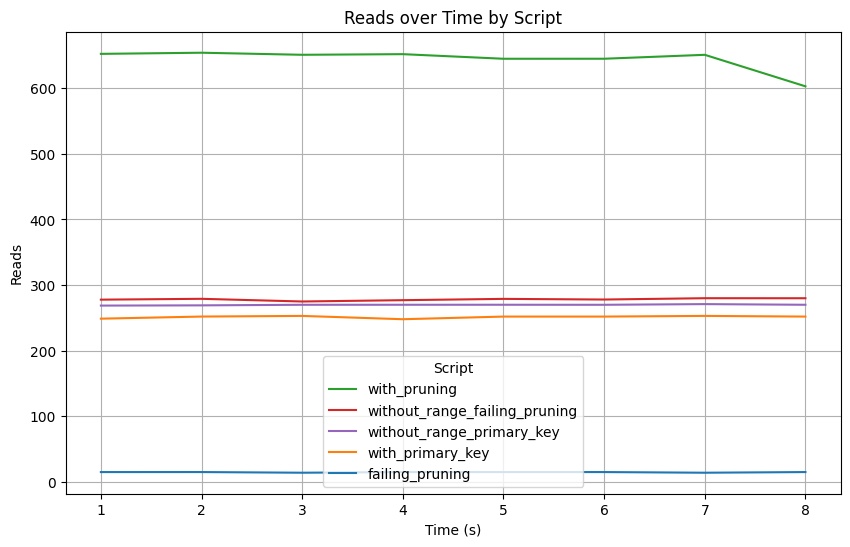
\includegraphics[width=\textwidth]{PNGs/Script/Partition/range-partition/Reads}
	\end{subfigure}
	\hfill
	\begin{subfigure}[t]{0.48\textwidth}
		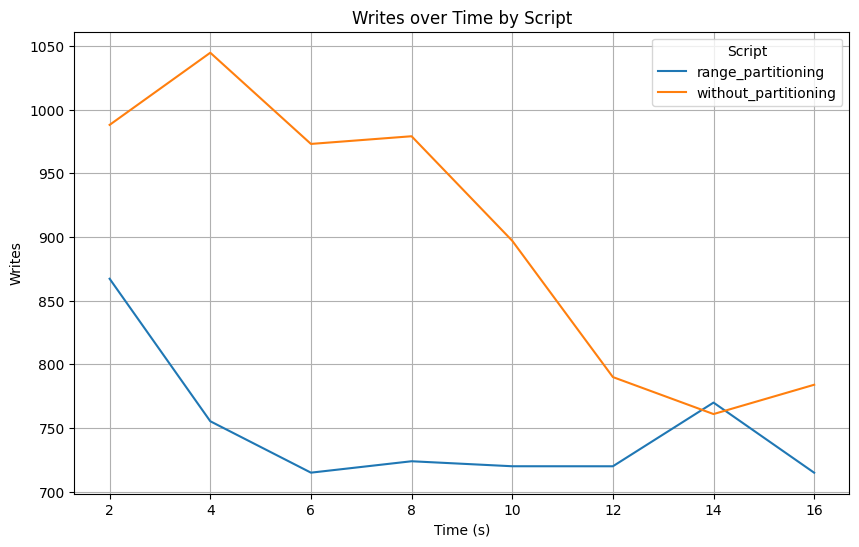
\includegraphics[width=\textwidth]{PNGs/Script/Partition/range-partition/Writes}
	\end{subfigure}
	\vspace{-9pt}
	\caption[Range-Partitionierung: Unterschiedliche Selects mit und ohne Partition]{Vergleich zwischen der Range-Partitionierung und ohne Partition}
	\label{fig:range-partition}
\end{figure}
\vspace{-19pt}

Bei der List-Partitionierung~\ref{fig:list-partition} können ebenfalls einige interessante Beobachtungen gemacht werden.
Beim ersten Fall ist nur ein Land in der WHERE-Bedingung vorhanden.
Wenn dies so ist, dann hat die Partitionierung einen erheblichen Vorteil gegenüber der Version ohne Partitionierung (siehe rote Linie von \texttt{with\_pruning\_simple} und braune von \texttt{without\_list\_pruning\_simple}).
Wenn statt nur eines Landes mehrere abgefragt werden, zeigen sich für die verschiedenen Operatoren unterschiedliche Ergebnisse.
Die beste Performance erzielt der IN-Operator.
Dicht darauf folgt der OR-Operator, während der Fall ohne Partitionierung mit etwas größerem Abstand kommt.
Deutlich abgeschlagen ist die Verbindung der Ergebnisse mit dem UNION-Operator.
Die Performance beim Einfügen der Daten ist bei der Partitionierung und dem Referenzfall sehr ähnlich, wobei letzterer einen leichten Vorteil hat.

\vspace{-7pt}
\begin{figure}[H]
	\centering
	\begin{subfigure}[t]{0.48\textwidth}
		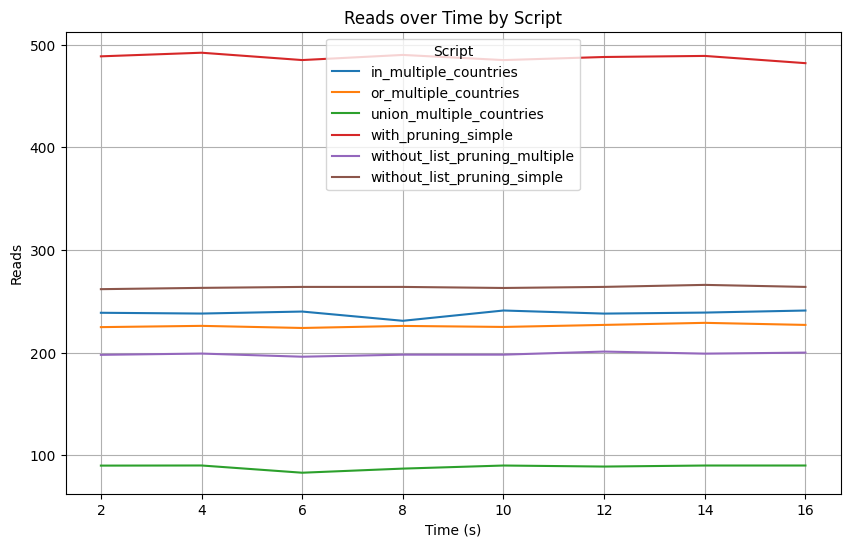
\includegraphics[width=\textwidth]{PNGs/Script/Partition/list-partition/Reads}
	\end{subfigure}
	\hfill
	\begin{subfigure}[t]{0.48\textwidth}
		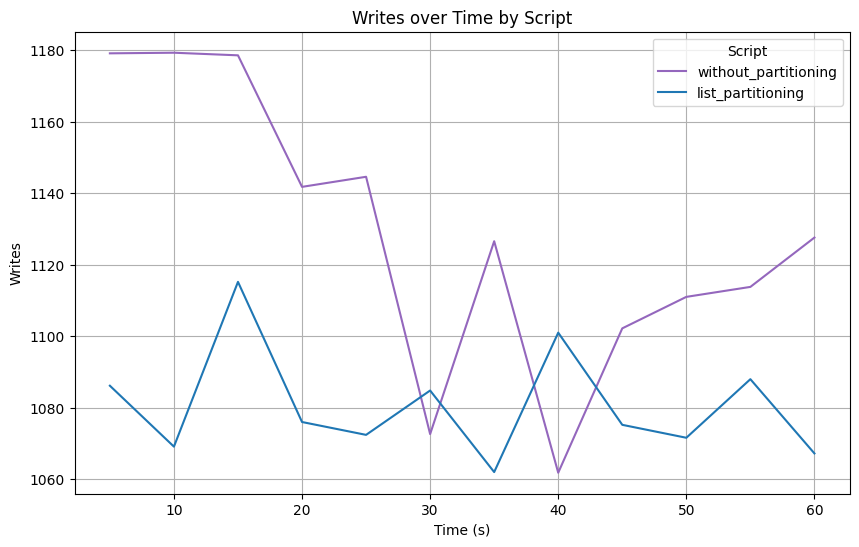
\includegraphics[width=\textwidth]{PNGs/Script/Partition/list-partition/Writes}
	\end{subfigure}
	\vspace{-9pt}
	\caption[List-Partitionierung: Unterschiedliche Abfragen mit und ohne Partition]{Vergleich zwischen der List-Partitionierung und ohne Partition}
	\label{fig:list-partition}
\end{figure}
\vspace{-19pt}

Bei der Key-Partitionierung fällt auf, dass es keinen signifikanten Performance-Unterschied zur Hash-Partitionierung gibt, sofern derselbe Datensatz und die gleiche Anzahl von Partitionen verwendet werden.
Generell ist die Key-Partitionierung häufig stabiler und optimierter ist, insbesondere wenn es um Primärschlüssel geht.
Bei der Hash-Partitionierung~\ref{fig:hash-partition} fällt auf, dass die Werte der Abfragen sehr konstant sind.
Nur bei der Variante mit 500 Partitionen gibt es deutlich sichtbare Schwankungen.
Diese liegen aber nicht an dem Pruning, denn mit dem SQL-Befehl \texttt{EXPLAIN} sehen wir, dass alle 500 Partitionen benötigt werden und keine Partitionen zufällig geprunt werden.
Die Hash-Partitionierung berechnet aus dem Wert einer bestimmten Spalte mithilfe einer Hash-Funktion einen Hash-Wert und anhand dessen wird die Zeile einer der Partitionen zugewiesen.
Da der Hash-Wert bei 500 Partitionen mit modulo 500 gebildet wird, landet jeder 500-ste Wert in der gleichen Partition.
Damit ist klargestellt, dass immer alle Partitionen benutzt werden, was die folgenden Ergebnisse zeigen.
Was die Performance angeht, zeigt sich, dass die Abfrage ohne Partitionierung am schnellsten ist.
Danach lässt sich die Regel ableiten, dass eine höhere Anzahl an Partitionen zu einer langsameren Abfrage führt.
Dies liegt daran, dass mehr Partitionen die Suche innerhalb der Struktur komplexer machen und dadurch die Performance beeinträchtigen.
Der Unterschied zwischen ohne Partitionen und 5 Partitionen ist noch überschaubar, aber bei 500 Partitionen sieht man einen sehr deutlichen Unterschied.
Damit wurde die Regel aus dem Kapitel~\ref{sec:partition-grundlagen} bestätigt.

\vspace{-4pt}
\begin{figure}[H]
	\centering
	\begin{subfigure}[t]{0.48\textwidth}
		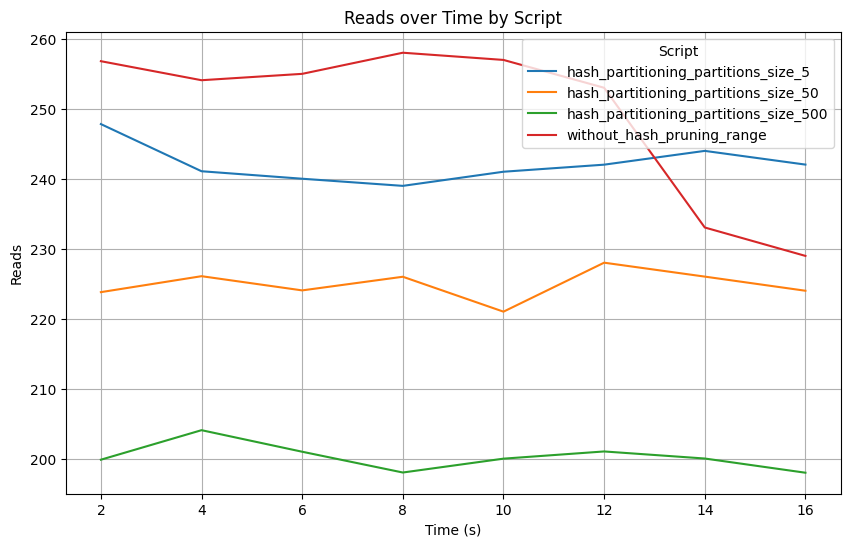
\includegraphics[width=\textwidth]{PNGs/Script/Partition/hash-partition/Reads}
	\end{subfigure}
	\hfill
	\begin{subfigure}[t]{0.48\textwidth}
		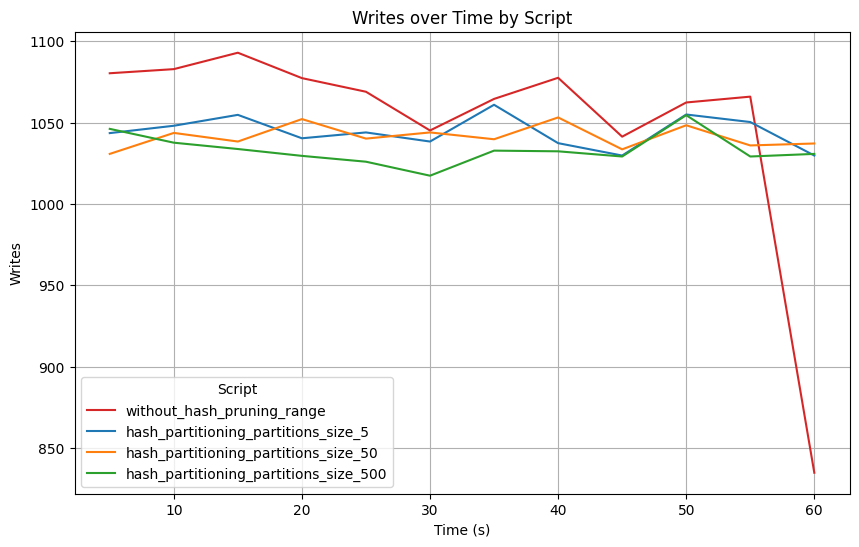
\includegraphics[width=\textwidth]{PNGs/Script/Partition/hash-partition/Writes}
	\end{subfigure}
	\vspace{-9pt}
	\caption[Hash-Partitionierung: Variationen der Partitionsanzahl]{Vergleich zwischen der Hash-Partitionierung und ohne Partition}
	\label{fig:hash-partition}
\end{figure}